\documentclass[letterpaper,10pt]{article}
\usepackage[top=2cm, bottom=1.5cm, left=1cm, right=1cm]{geometry}
\usepackage{amsmath, amssymb, amsthm,graphicx}
\usepackage{fancyhdr}
\pagestyle{fancy}

\lhead{\today}
\chead{Regression Assignment 6b}
\rhead{Justin Hood}

\newcommand{\Z}{\mathbb{Z}}
\newcommand{\Q}{\mathbb{Q}}
\newcommand{\R}{\mathbb{R}}
\newcommand{\C}{\mathbb{C}}
\newtheorem{lem}{Lemma}

\begin{document}
\begin{enumerate}
\item We consider the first-order autocorrelation of the Energy bills data. First, we consider the first order model of $y^*=\bar{y}$. Here, we now consider the equation for the test statistic,
\[d=\frac{\sum_{t=2}^n(e_t-e_{t-1})^2}{\sum_{t=1}^ne_t^2}\]
Here, $e_t$ is the the $t^{th}$ residual of the model. When we compute this as above, we get the $R$ output of
\[d=0.3908\]
Using the built in ACF function in $R$, we obtain the following plot,
\begin{center}
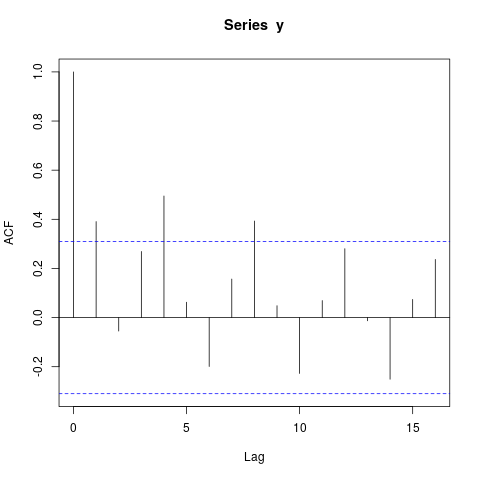
\includegraphics[scale=0.8]{acf.png}
\end{center}
Next, we compute a linear model of energy cost as a function of time. This model will then be used to compute the residuals for the purposes of a first order test. We compute $d$ as above to be equal to, $d=1.369812$. So, we test the hypotheses,
\[H_0: \text{The error is not autocorrelated}\]
\[H_A: \text{The error terms are positively autocorrelated}\]
With our computed $d$ statistic, we arrive at the $p$ value of $p=0.01266$ which falls below our threshold of $\alpha=0.05$. Thus, we reject our null hypothesis in favor of the alternative. So, we conclude that the data has positive first order autocorrelation.
\item Because our error terms are autocorrelated, we consider the following model,
\[y^*_t=\beta_0+\beta_1t+\beta_2t^2+\beta_3Q_2+\beta_4Q_3+\beta_5Q_4+\epsilon_t\]
Using $ARIMA$ in $R$, we obtain point estimates of $b_i$ and $\phi_1$.The results follow:
\begin{center}
\begin{tabular}{|c|c|}
\hline
Estimator & Estimate\\\hline
$b_0$ & $335.5962844$\\
$b_1$ & $-7.8140844$\\
$b_2$ & $0.3307836$\\
$b_3$ & $-104.7870853$\\
$b_4$ & $-195.5459704$\\
$b_5$ & $-68.8726069$\\
$\phi$ & $0.5890558$ \\\hline
\end{tabular}
\end{center}
\item We now compute the point prediction and prediction intervals of $y_{41}$ and $y_{42}$. First, we compute,
\[s=\sqrt{\frac{\sum y_i-\bar{y}}{n-1}}=111.666\]
Our computations are then as follows:
\[y_{41}=335.5962844-7.8140844(41)+0.3307836(41)^2+0.5890558*37.39=593.29\]
\[y_{42}=335.5962844-7.8140844(42)+0.3307836(42)^2-104.7870853(1)+0.5890558*37.39=508.145\]
Our intervals are then,
\[I_{41}=[y_{41}\pm z_{.025}*s]=[593.29\pm 1.96(111.666)]=[374.42464,\ 812.155]\]
\[I_{42}=[y_{42}\pm z_{.025}*s\sqrt{1+\phi^2}]=[254.130,\ 762.159]\]
\end{enumerate}
\end{document}
